%%%%%%%%%%%%%%%%%%%%%%%%%%%%%%%%%%%%%%%%%%%%%%%%%%%%%%%%%%%%%%%%%%%%%%%%%%%
\documentclass{article}
%%%%%%%%%%%%%%%%%%%%%%%%%%%%%%%%%%%%%%%%%%%%%%%%%%%%%%%%%%%%%%%%%%%%%%%%%%%

\usepackage{amssymb}
\usepackage{amsmath}
\usepackage{amsfonts}
\usepackage{amsthm}
\usepackage{graphicx}
\usepackage{tikz}
/Users/bubblyworld/Workspace/research/workspace/toolkit/bin/../assets/note_template/macros.tex

%%%%%%%%%%%%%%%%%%%%%%%%%%%%%%%%%%%%%%%%%%%%%%%%%%%%%%%%%%%%%%%%%%%%%%%%%%%
\begin{document}
%%%%%%%%%%%%%%%%%%%%%%%%%%%%%%%%%%%%%%%%%%%%%%%%%%%%%%%%%%%%%%%%%%%%%%%%%%%

\title{Territory and Conquest}
\author{Braden do Perez, Guy Paterson-Jones}

\maketitle

\begin{abstract}
  A study of a dynamical system on graphs that models territory control and conquest, loosely based on the board game \emph{Risk}. Every vertex is controlled by one of two players (black and white), and at each turn a vertex can change ownership based on influence from neighbouring vertices. Despite having somewhat simple rules, we describe a number of elusive conjectures about these dyamical systems that we are unable to prove. \cite{KrausEtAl1990}
\end{abstract}

%%%%%%%%%%%%%%%%%%%%%%%%%%%%%%%%%%%%%%%%%%%%%%%%%%%%%%%%%%%%%%%%%%%%%%%%%%%
\section{Introduction}
%%%%%%%%%%%%%%%%%%%%%%%%%%%%%%%%%%%%%%%%%%%%%%%%%%%%%%%%%%%%%%%%%%%%%%%%%%%

In the board game \emph{Risk}, the world consists of a number of territories, which are connected to each other by borders and sea routes. Each player controls one or more of these territories by placing armies on them, and each turn players can use these armies to wrest control of neighbouring territories from their opponents. In the standard rule set, a player wins the game when they either control every territory, or all of their opponents resign.

In these notes, we describe a simplified graph-theoretic model of a game of Risk. The idea is to model the state of the game at a particular point in time as a \emph{labelled graph}, where vertices represent territories, edges represent the connections between territories, and the label (or \emph{colour}) of a vertex represents the player that owns it. A game turn is modelled by an \emph{update function}, which changes the colours of the graph's vertices according to the colours of their neighbours. For instance, if a white vertex is surrounded by many black vertices, then the update function will change the colour of the white vertex to black. The following diagram should make the idea clear:

\begin{center}
  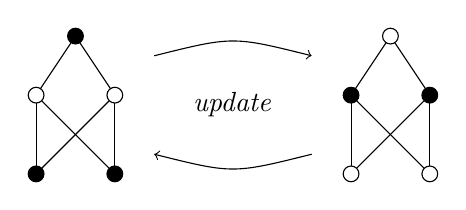
\begin{tikzpicture}
    % Leftmost graph:
    \draw (0,1) -- (0,0);
    \draw (1,1) -- (1,0);
    \draw (0,1) -- (1,0);
    \draw (1,1) -- (0,0);
    \draw (0.5,1.75) -- (0,1);
    \draw (0.5,1.75) -- (1,1);
    \filldraw[fill=black] (0.5,1.75) circle (0.1);
    \filldraw[fill=black] (0,0) circle (0.1);
    \filldraw[fill=white] (0,1) circle (0.1);
    \filldraw[fill=black] (1,0) circle (0.1);
    \filldraw[fill=white] (1,1) circle (0.1);

    % Rightmost graph:
    \draw (4,1) -- (4,0);
    \draw (5,1) -- (5,0);
    \draw (4,1) -- (5,0);
    \draw (5,1) -- (4,0);
    \draw (4.5,1.75) -- (4,1);
    \draw (4.5,1.75) -- (5,1);
    \filldraw[fill=white] (4.5,1.75) circle (0.1);
    \filldraw[fill=white] (4,0) circle (0.1);
    \filldraw[fill=black] (4,1) circle (0.1);
    \filldraw[fill=white] (5,0) circle (0.1);
    \filldraw[fill=black] (5,1) circle (0.1);

    % Update function arrows:
    \draw[->] (1.5,1.5) .. controls (2.5,1.75) .. (3.5,1.5);
    \draw[<-] (1.5,0.25) .. controls (2.5,0) .. (3.5,0.25);
    \draw (2.5,0.875) node {\emph{update}};
  \end{tikzpicture}
\end{center}

For simplicity, we will focus on the version of the model with two players, represented by the colours black and white. Nevertheless, the model hides a surprising amount of complexity. For instance, if one takes any finite black/white labelled graph and repeatedly applies the update function to it, one of two things eventually happens:

\begin{enumerate}
  \item The graph becomes monochromatic, i.e. one of the players wins.
  \item The graph settles into a periodic cycle, i.e. the same states keep occuring.
\end{enumerate}

The example we drew above is a periodic cycle of length $2$, since applying the update function repeatedly just alternates between the two graphs. In fact, \emph{every} case of a periodic cycle we've managed to come up with has length $2$! This leads us to conjecture that $2$ is the only possible length for a periodic cycle on a finite graph, but to date we have been unable to prove this.

%%%%%%%%%%%%%%%%%%%%%%%%%%%%%%%%%%%%%%%%%%%%%%%%%%%%%%%%%%%%%%%%%%%%%%%%%%%
\section{Choosing the Rules}
%%%%%%%%%%%%%%%%%%%%%%%%%%%%%%%%%%%%%%%%%%%%%%%%%%%%%%%%%%%%%%%%%%%%%%%%%%%

\newcommand{\selfDef}{\textsc{Sd}}
\newcommand{\nselfDef}{\neg \textsc{Sd}}
\newcommand{\tieNeu}{\textsc{Neu}}
\newcommand{\ntieNeu}{\neg \textsc{Neu}}

The main intuition we want to capture is that a vertex changes colour whenever its neighbourhood contains more \emph{enemies} than \emph{allies}. This raises (at least) two questions about the specifics of the update function:

\begin{enumerate}
  \item Does the vertex itself count as an allie? (``\emph{self-defence}'')
  \item What happens in the event of a tie? (``\emph{tie-breaking}'')
\end{enumerate}

Each of these questions leads to two obvious choices, for a total of four possible update functions. In the case of self-defence, we can either decide that a vertex \emph{does} count as its own allie (denoted $\selfDef$), or that it \emph{doesn't} count as its own allie (denoted $\nselfDef$). In the case of tie-breaking, we can either decide that a tied vertex becomes \emph{neutral} (i.e. owned by nobody, denoted $\tieNeu$), or that it simply stays the \emph{same} colour (denoted $\ntieNeu$).

The four combinations are then $\selfDef \wedge \tieNeu$, $\selfDef \wedge \ntieNeu$, $\nselfDef \wedge \tieNeu$ and $\nselfDef \wedge \ntieNeu$. To decide which of these combinations is the most natural, we look at what happens when we update the simplest possible black/white coloured graph according to these rules:

\begin{center}
  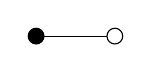
\begin{tikzpicture}
    \draw (0,0) -- (1,0);
    \filldraw[fill=black] (0,0) circle (0.1);
    \filldraw[fill=white] (1,0) circle (0.1);
  \end{tikzpicture}
\end{center}

\begin{center}
  \begin{tabular}{c|c|c|}
    \multicolumn{1}{c}{} &
    \multicolumn{1}{c}{$\selfDef$} &
    \multicolumn{1}{c}{$\nselfDef$} \\ 
    \cline{2-3}
    $\tieNeu$ &
    
    \begin{tikzpicture}
      \draw[fill=white,white] (-1, -1) rectangle (2, 1);
      \draw (0,0) -- (1,0);
      \filldraw[fill=gray] (0,0) circle (0.1);
      \filldraw[fill=gray] (1,0) circle (0.1);
    \end{tikzpicture} &

    \begin{tikzpicture}
      \draw[fill=white,white] (-1, -1) rectangle (2, 1);
      \draw (0,0) -- (1,0);
      \filldraw[fill=white] (0,0) circle (0.1);
      \filldraw[fill=black] (1,0) circle (0.1);
    \end{tikzpicture} \\

    \cline{2-3}
    $\ntieNeu$ &

    \begin{tikzpicture}
      \draw[fill=white,white] (-1, -1) rectangle (2, 1);
      \draw (0,0) -- (1,0);
      \filldraw[fill=black] (0,0) circle (0.1);
      \filldraw[fill=white] (1,0) circle (0.1);
    \end{tikzpicture} &

    \begin{tikzpicture}
      \draw[fill=white,white] (-1, -1) rectangle (2, 1);
      \draw (0,0) -- (1,0);
      \filldraw[fill=white] (0,0) circle (0.1);
      \filldraw[fill=black] (1,0) circle (0.1);
    \end{tikzpicture} \\

    \cline{2-3}
  \end{tabular}
\end{center}

%%%%%%%%%%%%%%%%%%%%%%%%%%%%%%%%%%%%%%%%%%%%%%%%%%%%%%%%%%%%%%%%%%%%%%%%%%%
\section{Notation}
%%%%%%%%%%%%%%%%%%%%%%%%%%%%%%%%%%%%%%%%%%%%%%%%%%%%%%%%%%%%%%%%%%%%%%%%%%%

%%%%%%%%%%%%%%%%%%%%%%%%%%%%%%%%%%%%%%%%%%%%%%%%%%%%%%%%%%%%%%%%%%%%%%%%%%%
\bibliographystyle{unsrt}
\bibliography{bibliography}
%%%%%%%%%%%%%%%%%%%%%%%%%%%%%%%%%%%%%%%%%%%%%%%%%%%%%%%%%%%%%%%%%%%%%%%%%%%

%%%%%%%%%%%%%%%%%%%%%%%%%%%%%%%%%%%%%%%%%%%%%%%%%%%%%%%%%%%%%%%%%%%%%%%%%%%
\end{document}
%%%%%%%%%%%%%%%%%%%%%%%%%%%%%%%%%%%%%%%%%%%%%%%%%%%%%%%%%%%%%%%%%%%%%%%%%%%
